\documentclass{beamer}

\usepackage{graphicx}
\usepackage[sfdefault,light]{FiraSans}
%\usefonttheme{serif} 
\usepackage[british]{datetime2}
\usetheme{default}
\setbeamertemplate{navigation symbols}{} % No navigation symbols
\setbeamercolor{alerted text}{fg=blue!80!green!159!}
\setbeamercolor{frame title}{fg=blue!80!green!159!}
\setbeamercolor{title}{fg=blue!80!green!159!}
\setbeamercolor{subtitle}{fg=blue!80!green!159!}

\makeatletter
\setbeamertemplate{footline}
{
  \leavevmode%
  \hbox{%
  \begin{beamercolorbox}[wd=.15\paperwidth,ht=2.25ex,dp=1ex,center]{institute in head/foot}%
    \usebeamerfont{title in head/foot}%
    \raisebox{-0.15cm}{
\includegraphics[width=1cm]{logo_ntnu_u-slagord.pdf}}
  \end{beamercolorbox}%
  \begin{beamercolorbox}[wd=.6\paperwidth,ht=2.25ex,dp=1ex,center]{institute in head/foot}%
    \usebeamerfont{title in head/foot}%
    \insertsection
  \end{beamercolorbox}%
  \begin{beamercolorbox}[wd=.15\paperwidth,ht=2.25ex,dp=1ex,center]{institute in head/foot}%
    \usebeamerfont{title in head/foot}%
    \insertshortdate
  \end{beamercolorbox}%
  \begin{beamercolorbox}[wd=.1\paperwidth,ht=2.25ex,dp=1ex,right]{institute in head/foot}%
    \usebeamerfont{title in head/foot} 
    \insertframenumber{} / \inserttotalframenumber\hspace*{2ex} 
  \end{beamercolorbox}}%
}
\makeatother

%----------------------------------------------------------------------------------------
%	TITLE PAGE
%----------------------------------------------------------------------------------------

\title{POL2012: Theories and Models in Political Economy}
\subtitle{Marxism}
% \date{\today}
\date{}
\author{Marius Swane Wishman}
\institute{Department of Sociology and Political Science}

\begin{document}

\begin{frame}[plain]
\titlepage % Print the title page as the first slide
\centering % Comment out if second logo

\includegraphics[width=5cm]{logo_ntnu_u-slagord.pdf}
%\hspace{0.5cm} 
\includegraphics[width=5cm]{logo_ntnu_u-slagord.pdf} % Second logo
\end{frame}


\section{Introduction} % Sections can be created in order to organize your presentation into discrete blocks, all sections and subsections are automatically printed in the table of contents as an overview of the talk
%------------------------------------------------
\begin{frame}{Introduction}
\begin{itemize}[<+- | alert@+>]
    \item Marxism $\neq$ Communism
    \item Marxism $\neq$ Political Marxism
    \item Marxism $\approx$ Grand theory $\approx$ Paradigm  $\approx$ Theoretical framework 
\end{itemize} 
\end{frame}{}

\section{Historical context}

\begin{frame}{Historical Context - A(nother) Crisis of Capitalism}
    \begin{figure}
        \centering
        \includegraphics[width = .8\textwidth]{../img/labor.jpg}
        \label{fig:labor}
    \end{figure}{}
\end{frame}

\begin{frame}{Karl Marx (1818-1883)}
              \begin{figure}
                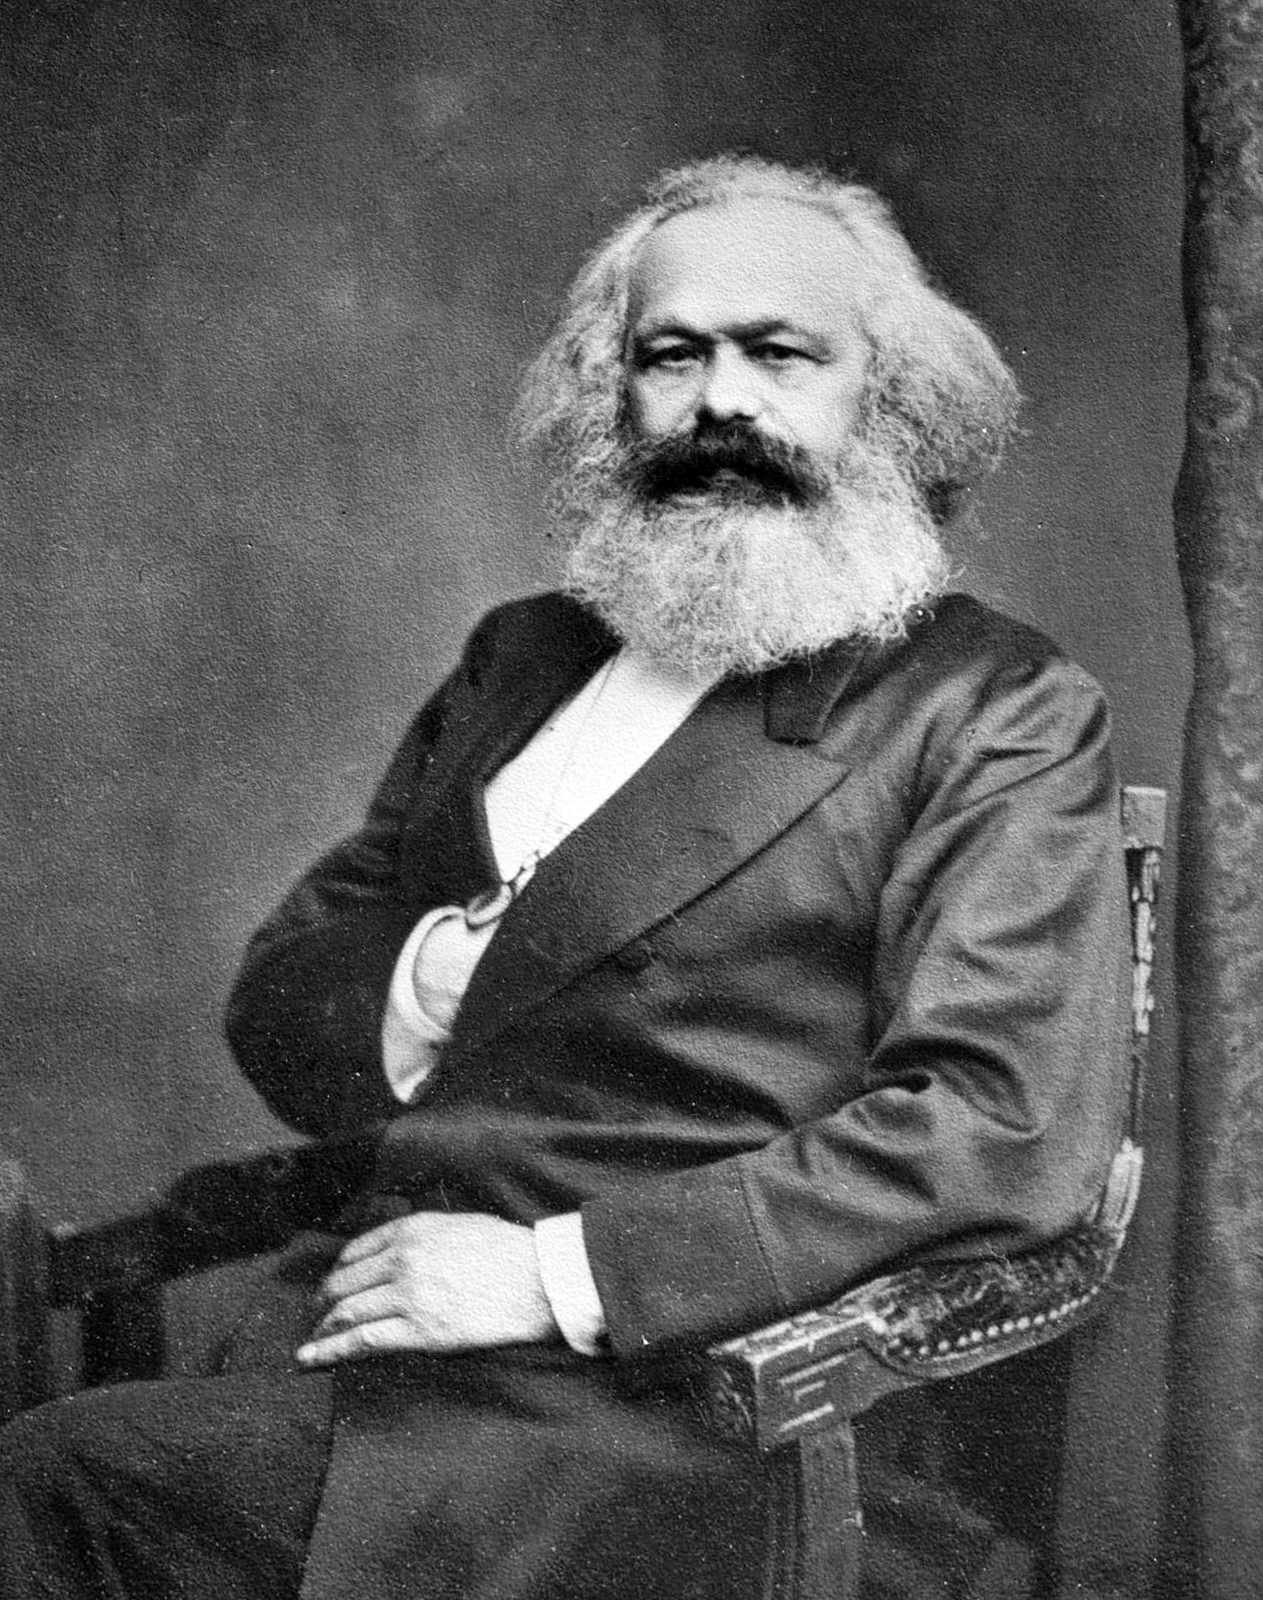
\includegraphics[width=.6\textwidth]{../img/karl.png}
                \label{fig:karl}
             \end{figure}{}
\end{frame}{}

\section{The method of Marx}

\begin{frame}{A new method}
    \begin{figure}
        \centering
        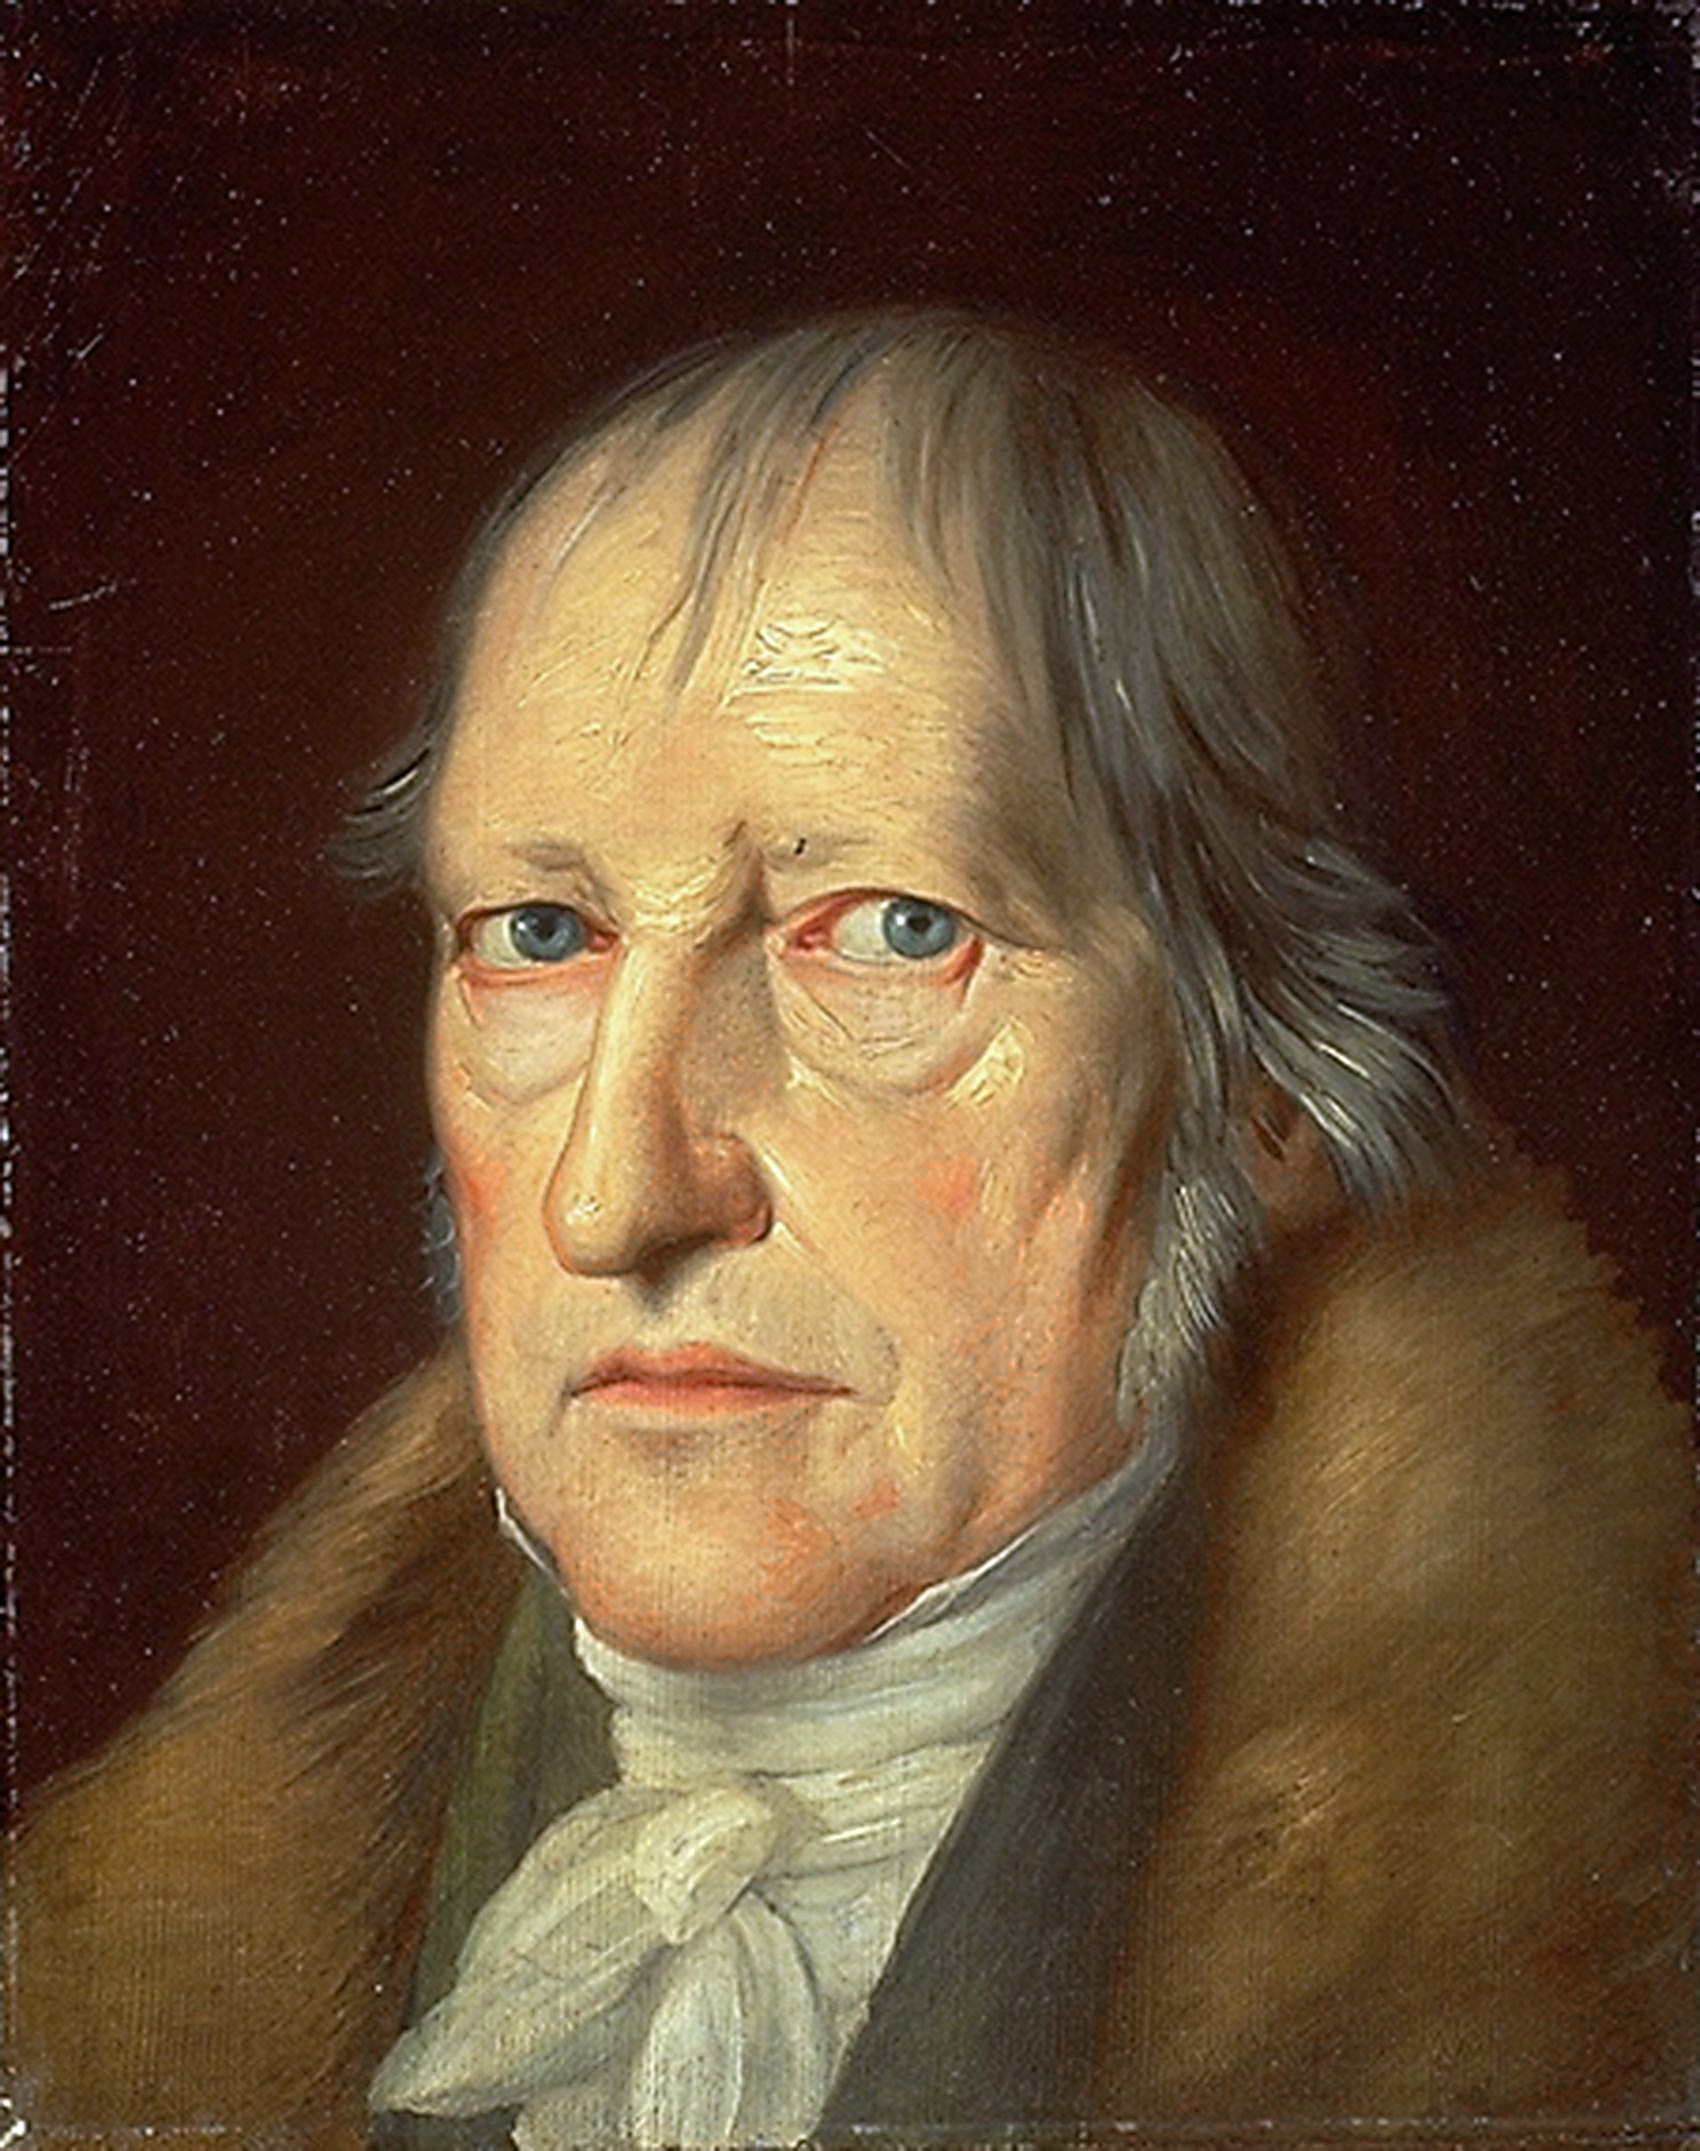
\includegraphics[width=.5\textwidth]{../img/Hegel_by_Schlesinger.jpg}
        \caption{Georg Wilhelm Friedrich Hegel}
        \label{fig:hegel}
    \end{figure}{}
\end{frame}{}

\section{The theory of Marx}
\begin{frame}{Criticism of capitalism} % He is focused on the system and society, not conserned with other thinkers
    \begin{figure}
        \centering
        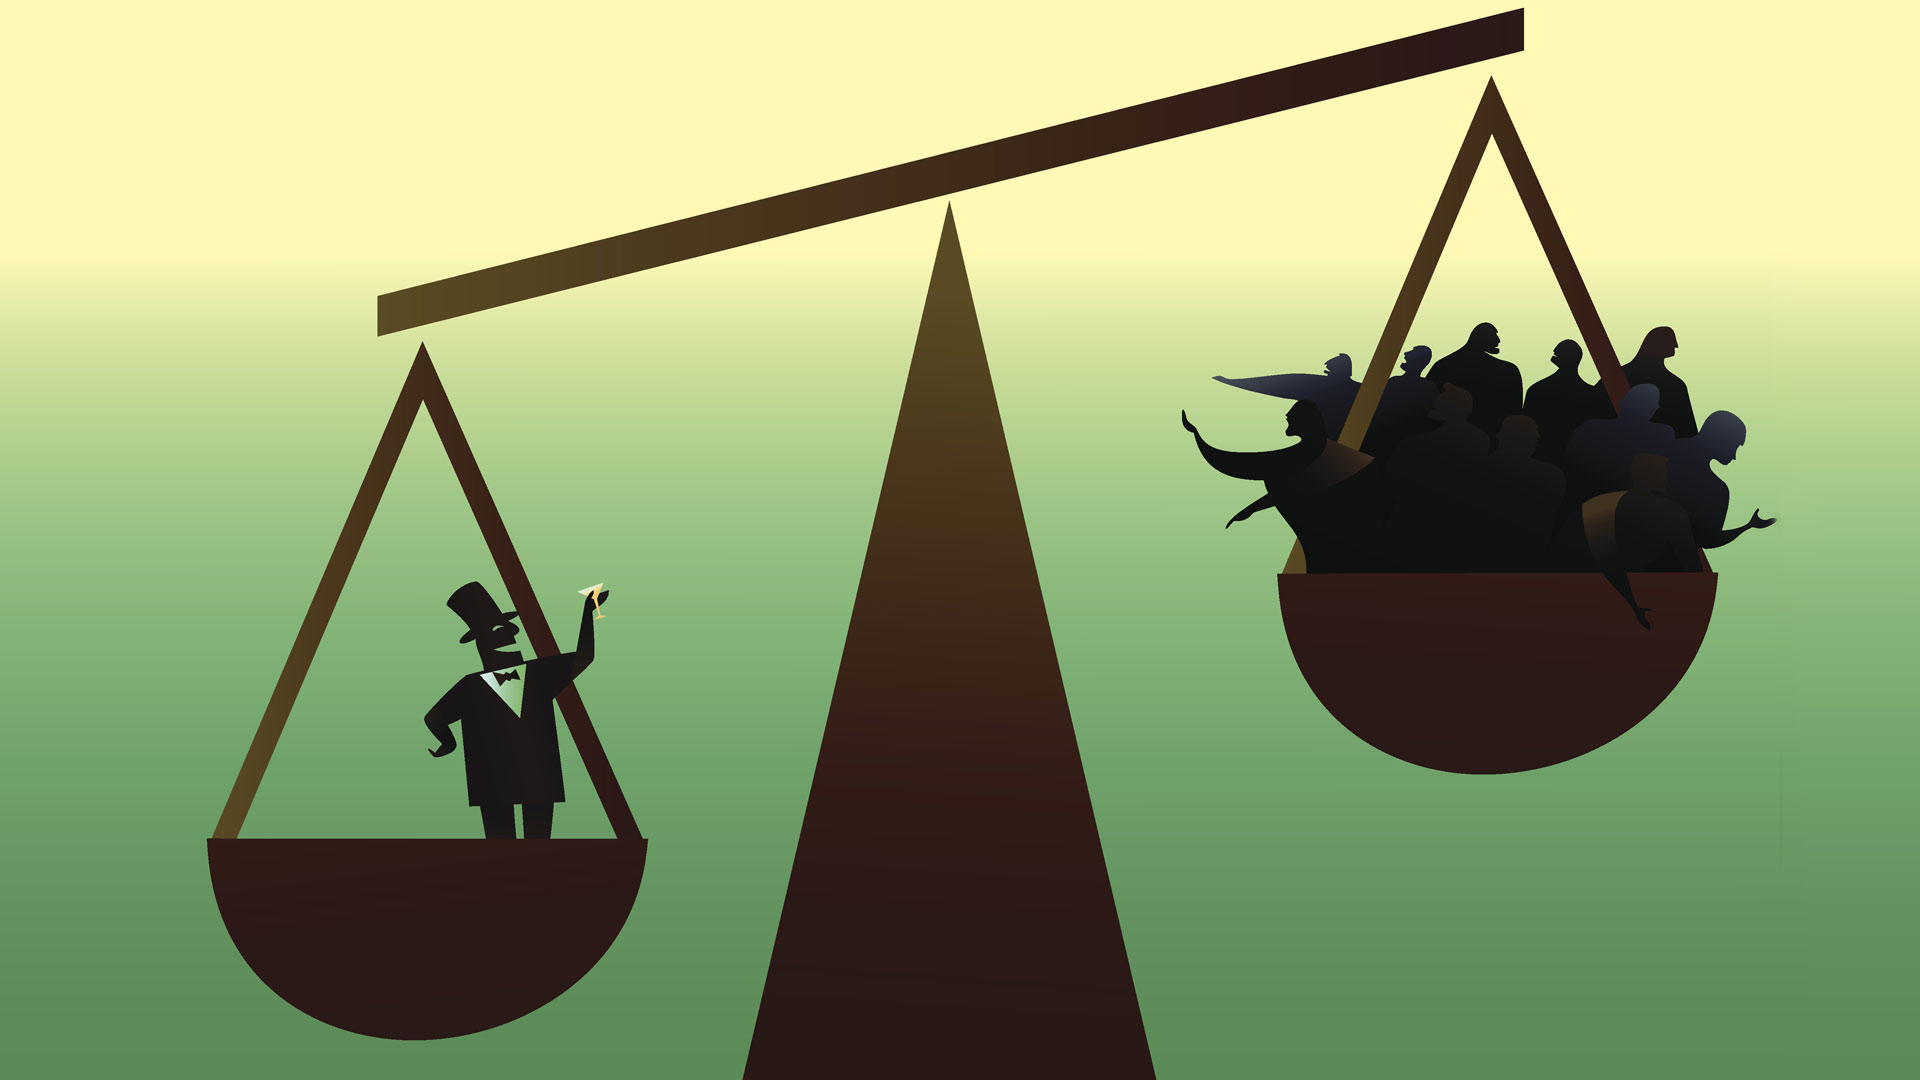
\includegraphics[width=\textwidth]{../img/class.jpg}
        \label{fig:class}
    \end{figure}{}
\end{frame}

\begin{frame}{Exploitation and the labor theory of value}

	\begin{figure}[htpb]
		\centering
		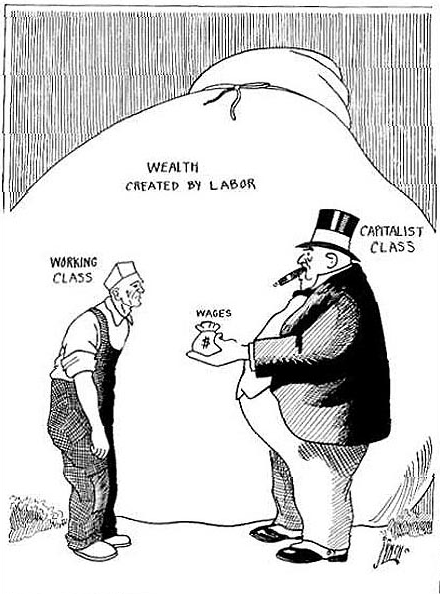
\includegraphics[width=0.6\linewidth]{../img/explot.png}
		\label{fig:exploit}
	\end{figure}

\end{frame}

\begin{frame}{Internal contradictions} 

	\begin{figure}[htpb]
		\centering
		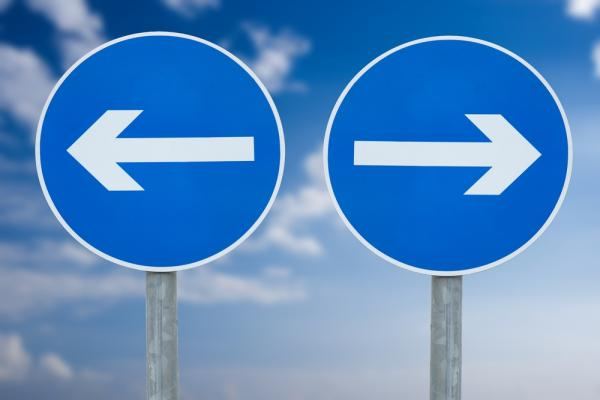
\includegraphics[width=0.8\linewidth]{../img/contradiction.jpg}
	\end{figure}

\end{frame}

\begin{frame}{Economic Crises}

	\begin{figure}[htpb]
		\centering
		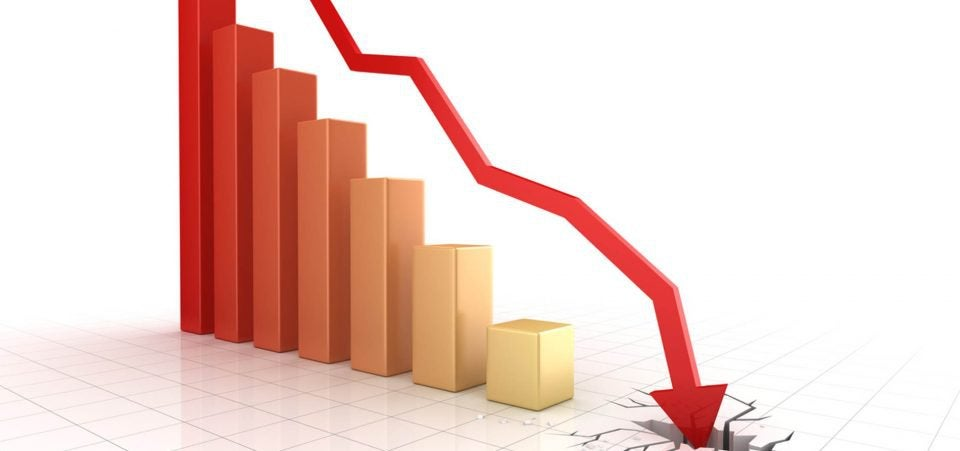
\includegraphics[width=0.8\linewidth]{../img/crash2.jpeg}
	\end{figure}

\end{frame}

\begin{frame}{The State}

	\begin{figure}[htpb]
		\centering
		\includegraphics[width=0.6\linewidth]{../img/Anti-capitalism_color—_Restored.png}
	\end{figure}

\end{frame}

\begin{frame}{But what about growth?}

\begin{figure}[htpb]
	\centering
	
\includegraphics[width=0.6\linewidth]{../img/monopoly.png}
\end{figure}	

\end{frame}
\section{Conclusion}

\begin{frame}{To the barricades!}

    \begin{figure}
        \centering
        \includegraphics[width=.8\textwidth]{../img/Delacroix.jpg}
        \label{fig:liberty}
    \end{figure}{}

\end{frame}

\begin{frame}{A word of caution}

	\begin{figure}[htpb]
		\centering
		
\includegraphics[width=0.8\linewidth]{../img/calm.jpg}
	\end{figure}

\end{frame}

\end{document} 

